\subsection{Autocorrelation study of the time sequence of sources of activity in the WLAN - Results} \label{sec:autocorrelation_active_results}

\subsubsection{Session Experiment - Results} \label{subsec:autocorrelation_sessions}
This experiment will study the session level influence in the independence of the active samples. Following a similar procedure as the one followed in Section \ref{sec:gv_session_exp}, we used different number of sessions with similar load and studied the autocorrelation function of the active samples of each one of the cases. The flow level (size, inter-arrival) configuration is fixed and we randomized the packet level with the following configuration:

\begin{itemize}
\item Packet Size distribution: A uniform packet distribution with a normal average [e.g. 768 bytes] for all flows and for all sessions.
\item An exponential packet inter-arrival time distribution with some practical mean [e.g. 100 ms] for all flows and for all sessions.
\end{itemize}

The final configuration for the different levels of the Extended Multi-Layer traffic model is presented in Table \ref{tab:sim_traffic_model}. We selected three session cases, i.e. 5, 10 and 20 sessions with a load of around 20 \%.

The independence of the active samples is studied using the autocorrelation function. The autocorrelation function will determine the correlation of the sequence of samples and will give us an evaluation on how independent are the consecutive active periods. We have extracted the sequence of active periods (just focusing on the DATA packets) from the traffic generated with the extended multi-layer traffic model which contains which stations (\acs{WLAN} users) had sent the active period. We have obtained the autocorrelation from this sequence of stations. These results are represented in Figure \ref{fig:autocorrelation_sessions}.

\begin{figure}[h!]
	\centering
	\subfloat[]{
		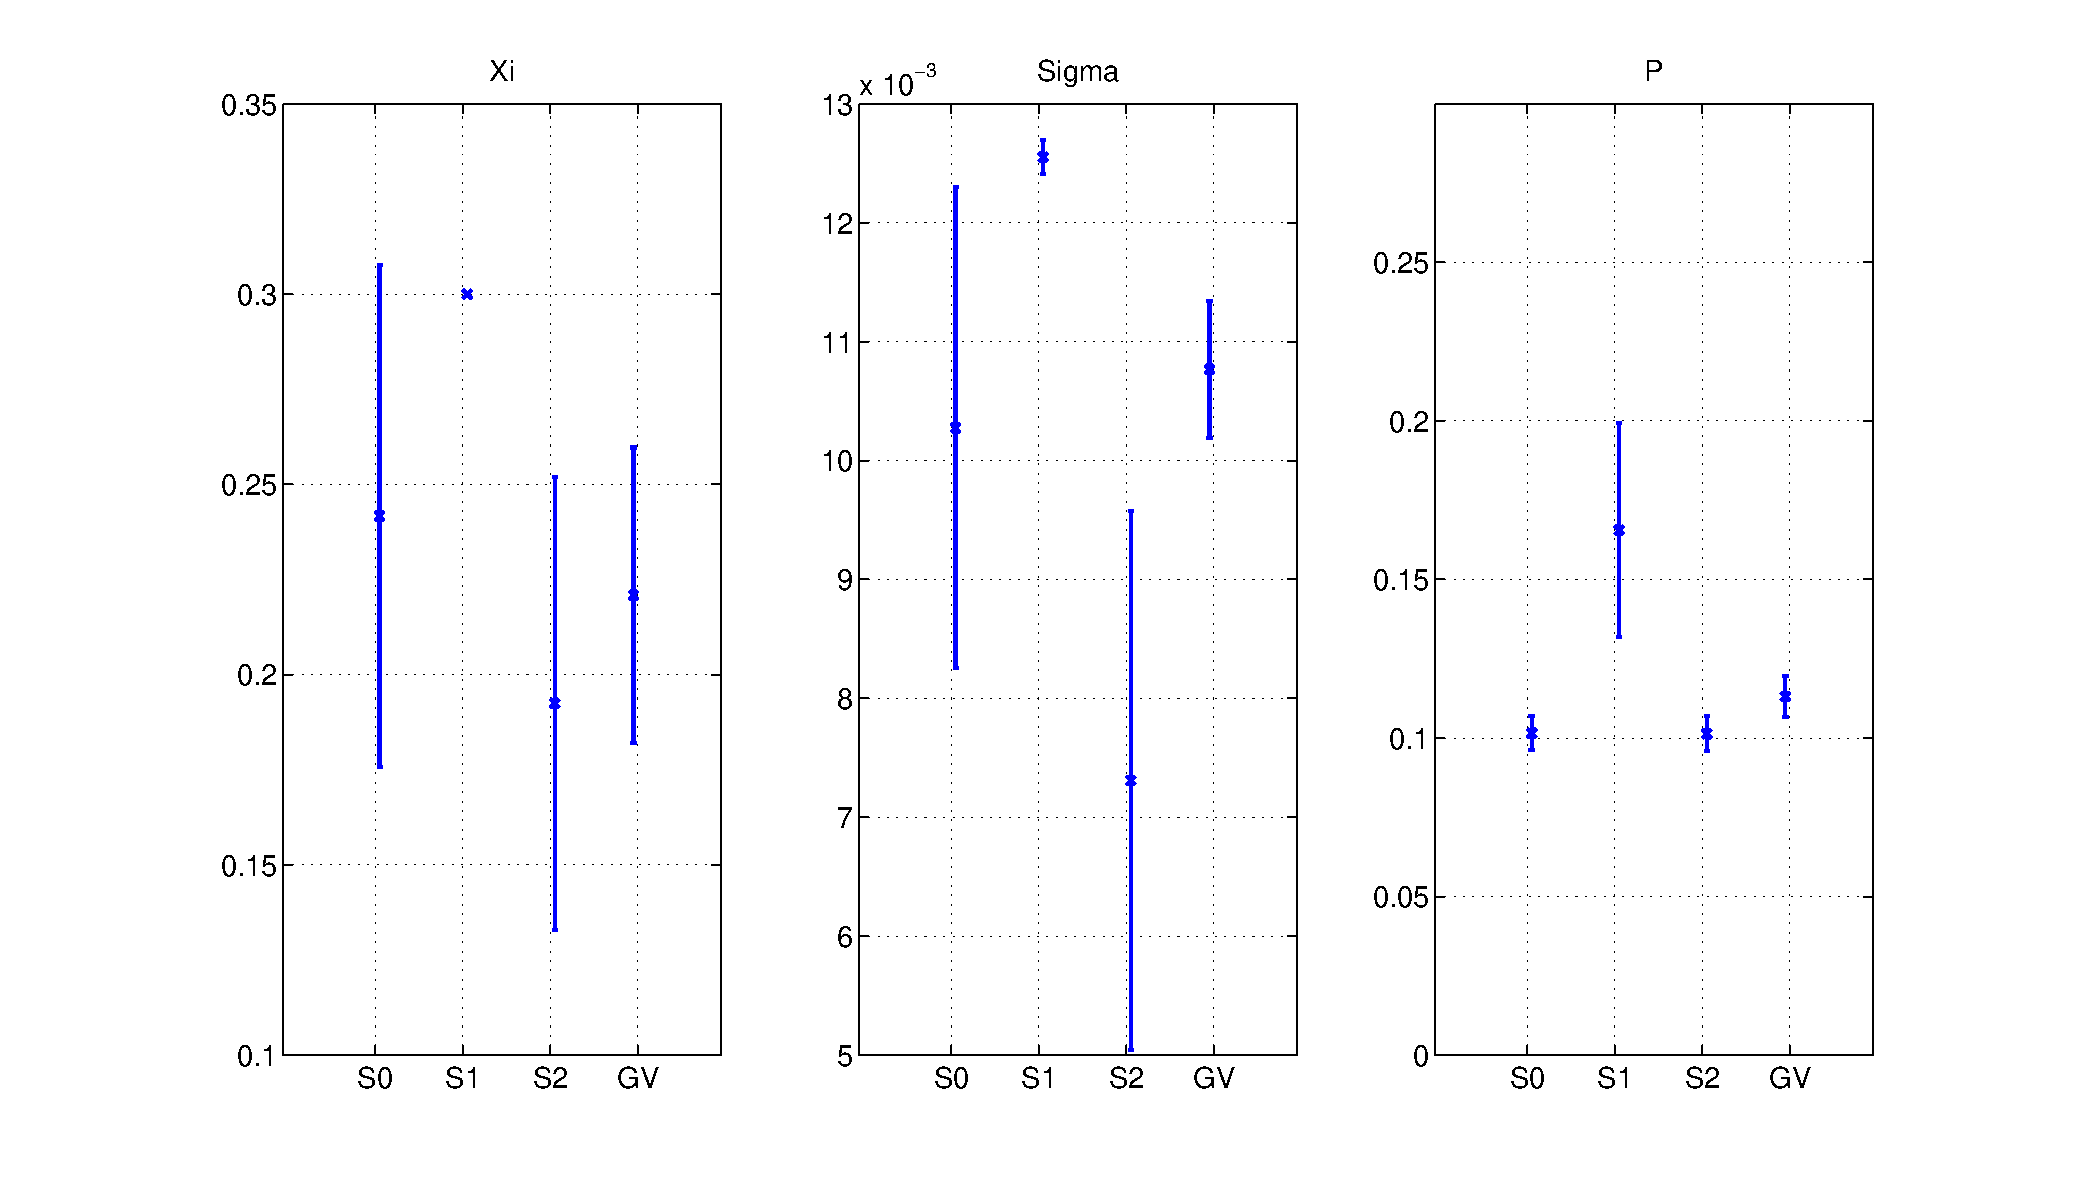
\includegraphics[width=0.33\textwidth, trim = 0mm 0mm 0mm 0mm, clip]{images/results/autocorrelation/sessions/5sessions}
		\label{fig:autocorrelation_2sessions}
	}
	\subfloat[]{
		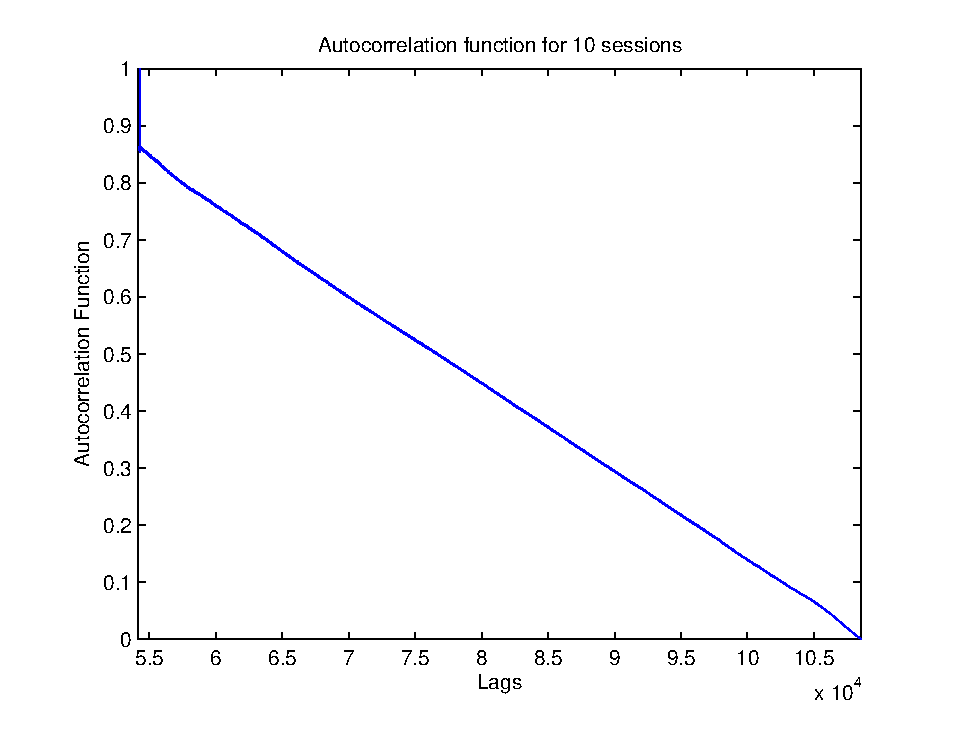
\includegraphics[width=0.33\textwidth, trim = 0mm 0mm 0mm 0mm, clip]{images/results/autocorrelation/sessions/10sessions}
		\label{fig:autocorrelation_12sessions}
	}
	\subfloat[]{
		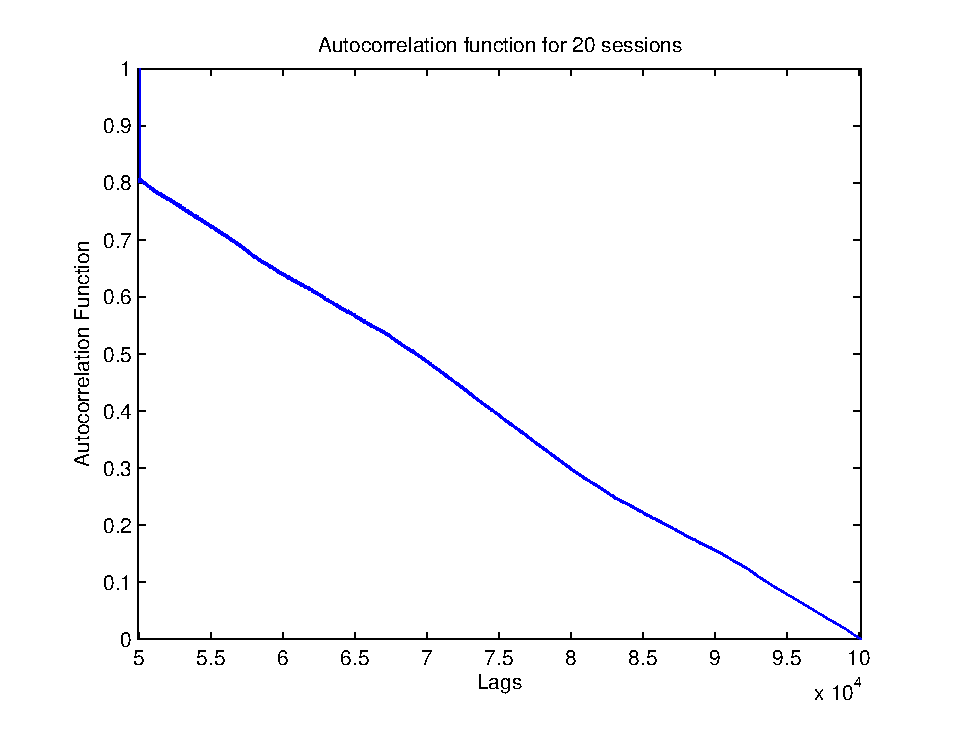
\includegraphics[width=0.33\textwidth, trim = 0mm 0mm 0mm 0mm, clip]{images/results/autocorrelation/sessions/20sessions}
		\label{fig:autocorrelation_20sessions}
	}
	\caption{Autocorrelation function of the different sources of DATA packets for different number of sessions with similar load. The correlation between samples is reduced for higher number of sources.}
	\label{fig:autocorrelation_sessions}
\end{figure}

In Figure \ref{fig:autocorrelation_sessions} we plotted the autocorrelation function for three different number of sessions cases and similar load in order to compare them. An independent sequence is represented by an autocorrelation function that is approximated by a $\delta$. As it can be observed, there is an improvement in the independence of the active periods when the number of sessions is higher. It is clear that the higher is the number of sessions, more random will be the access to the medium of the different stations of in the network. It is possible to conclude from this experiment that the session number decreases the correlation between the samples. However it is not possible to conclude that consecutive active periods are totally independent as it has been assumed in the Local View model.

\subsubsection{In-Session Experiment - Results} \label{subsec:autocorrelation_insessions}
Once we tested the effect of the session number in the independence of the sequence of active samples, it is necessary to study how the load affects this independence. In this case, we repeated the experiments using a determined number of sessions (10 \acs{WLAN} users) and we randomized the flow and packet levels and extracted again the autocorrelation function from the stations sequence. The configuration of the different levels of the extended multi-layer traffic model can be found in Table \ref{tab:sim_traffic_model} and the packet level is configured as it was done in the previous experiment. The results of this experiment are represented in Figure \ref{fig:autocorrelation_insessions}.

\begin{figure}[h!]
	\centering
	\subfloat[14.2581249 \%]{
		\includegraphics[width=0.5\textwidth, trim = 0mm 0mm 0mm 0mm, clip]{images/results/autocorrelation/load/14}
		\label{fig:autocorrelation_load14}
	}
	\subfloat[21.474477 \%]{
		\includegraphics[width=0.5\textwidth, trim = 0mm 0mm 0mm 0mm, clip]{images/results/autocorrelation/load/21}
		\label{fig:autocorrelation_load21}
	}\\
	\subfloat[37.280606 \%]{
		\includegraphics[width=0.5\textwidth, trim = 0mm 0mm 0mm 0mm, clip]{images/results/autocorrelation/load/37}
		\label{fig:autocorrelation_load37}
	}
	\subfloat[49.485722 \%]{
		\includegraphics[width=0.5\textwidth, trim = 0mm 0mm 0mm 0mm, clip]{images/results/autocorrelation/load/49}
		\label{fig:autocorrelation_load49}
	}
	\caption{Autocorrelation function for 10 sessions for different load cases}
	\label{fig:autocorrelation_insessions}
\end{figure}

From the results of this experiment, it can be observed that the load has a slight effect in the autocorrelation function and, in extension, the independence of the samples. It can be observed how the autocorrelation function tends to a delta function for higher loads. It can be concluded then, that the increase in the load is translated in a higher independence of the samples. When the network is saturated this independence is almost perfect because of the high random access of the packets to the medium. However, the improvement is not that critical as the one presented in the Session experiment.

With the autocorrelation experiments developed in this section, we have shown that the active samples can be considered independent enough, so the assumption in the semi-Markovian model that consecutive active periods are independent has been proved and we will continue with the study of the Local View model in the next chapter.